\documentclass[journal]{IEEEtran}
\usepackage[a5paper, margin=10mm, onecolumn]{geometry}
\usepackage{lmodern}
\usepackage{tfrupee}
\setlength{\headheight}{1cm}
\setlength{\headsep}{0mm}

\usepackage{gvv-book}
\usepackage{gvv}
\usepackage{cite}
\usepackage{amsmath,amssymb,amsfonts,amsthm}
\usepackage{algorithmic}
\usepackage{graphicx}
\usepackage{textcomp}
\usepackage{xcolor}
\usepackage{txfonts}
\usepackage{listings}
\usepackage{enumitem}
\usepackage{mathtools}
\usepackage{gensymb}
\usepackage{comment}
\usepackage[breaklinks=true]{hyperref}
\usepackage{tkz-euclide}
\usepackage{listings}
\def\inputGnumericTable{}
\usepackage[latin1]{inputenc}
\usepackage{color}
\usepackage{array}
\usepackage{longtable}
\usepackage{calc}
\usepackage{multirow}
\usepackage{hhline}
\usepackage{ifthen}
\usepackage{lscape}
\usepackage{xparse}

\bibliographystyle{IEEEtran}

\title{9.2.3}
\author{EE25BTECH11043 - Nishid Khandagre}

\begin{document}
\maketitle

\renewcommand{\thefigure}{\theenumi}
\renewcommand{\thetable}{\theenumi}

\numberwithin{equation}{enumi}
\numberwithin{figure}{enumi}

\textbf{Question}:
Draw a rough sketch of the given curve $y = 1 + |x + 1|$, $x = -3$, $x = 3$, $y = 0$, and
find the area of the region bounded by them, using integration.

\textbf{Solution: }
Given the curve $y = 1 + |x + 1|$.
\begin{itemize}
    \item For $x < -1$: $|x+1| = -(x+1)$.
    \begin{align}
        y &= 1 - (x+1) \\
        y &= -x
        \end{align}
        \begin{align}
        \myvec{1&1}\myvec{x\\y}=0
    \end{align}
    \item For $x \ge -1$: $|x+1| = x+1$.
    \begin{align}
        y &= 1 + (x+1) \\
        y &= x+2
        \end{align}
        \begin{align}
        \myvec{1&-1}\myvec{x\\y}=-2
    \end{align}
\end{itemize}

At $x=-3$: $y = -(-3) = 3$.

At $x=-1$: For $y=-x$, $y=1$. For $y=x+2$, $y=(-1)+2=1$.\\Both pieces meet at $\myvec{-1\\1}$.

At $x=3$: $y = 3+2 = 5$.


The region is bounded by $y = -x$ from $\myvec{-3\\3}$ to $\myvec{-1\\1}$ and $y = x+2$ from $\myvec{-1\\1}$ to $\myvec{3\\5}$ and by the lines $x=-3$, $x=3$, and $y=0$.





\textbf{Area calculation for the left piece:}
For $y=-x$ 
\begin{align}
    \text{Area}_1 &= \int_{-3}^{-1} -x \,dx \\
    &= \myvec{-1 & 0} \left( \begin{pmatrix}\tfrac{x^2}{2} \\ x\end{pmatrix} \right) \Big|_{-3}^{-1} \\
    &= \left[ -\frac{x^2}{2} \right]_{-3}^{-1} \\
    &= -\frac{1}{2} + \frac{9}{2} \\
    &= 4
\end{align}

\textbf{Area calculation for the right piece:}
For $y=x+2$
\begin{align}
    \text{Area}_2 &= \int_{-1}^{3} (x+2) \,dx \\
    &= \myvec{1 & 2} \left( \begin{pmatrix}\tfrac{x^2}{2} \\ x\end{pmatrix} \right) \Big|_{-1}^{3} \\
    &= \left[ \frac{x^2}{2} + 2x \right]_{-1}^{3} \\
    &= \left( \frac{9}{2} + 6 \right) - \left( \frac{1}{2} - 2 \right) \\
    &= \frac{21}{2} + \frac{3}{2} \\
    &= 12
\end{align}

The total area is the sum of the areas of the two pieces.
\begin{align}
    \text{Total Area} &= \text{Area}_1 + \text{Area}_2 \\
    &= 4 + 12 \\
    &= 16
\end{align}

Thus, the total area of the region bounded by the curves is $16$ square units.

\begin{figure}[H]
\centering
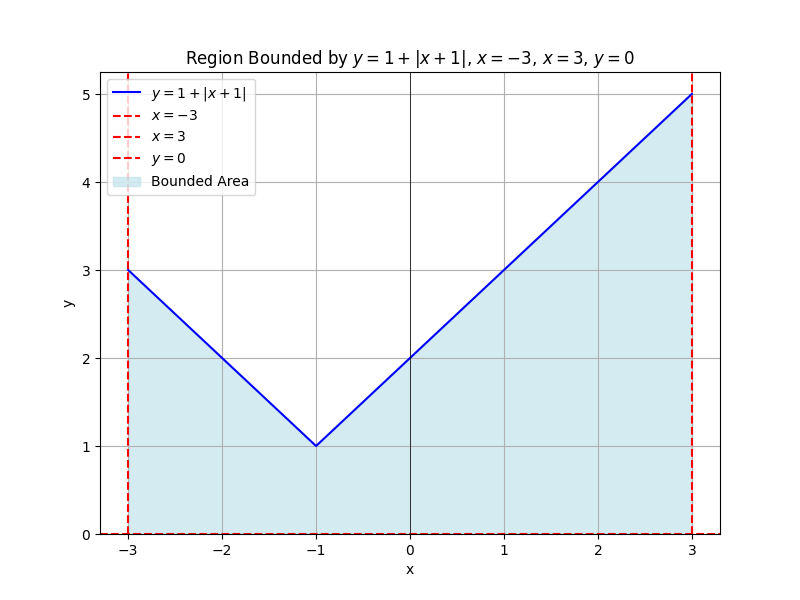
\includegraphics[width=0.7\columnwidth]{figs/fig2.png}
\caption{}
\label{fig:1}
\end{figure}
\end{document}
